\documentclass[12pt]{article}%
\usepackage{amsfonts}
\usepackage{fancyhdr}
\usepackage{comment}
\usepackage{listings}
\usepackage[a4paper, top=2.5cm, bottom=2.5cm, left=2.2cm, right=2.2cm]%
{geometry}
\usepackage{times}
\usepackage{amsmath}
\usepackage{changepage}
\usepackage{amssymb}
\usepackage{graphicx}%
\setcounter{MaxMatrixCols}{30}
\newtheorem{theorem}{Theorem}
\newtheorem{acknowledgement}[theorem]{Acknowledgement}
\newtheorem{algorithm}[theorem]{Algorithm}
\newtheorem{axiom}{Axiom}
\newtheorem{case}[theorem]{Case}
\newtheorem{claim}[theorem]{Claim}
\newtheorem{conclusion}[theorem]{Conclusion}
\newtheorem{condition}[theorem]{Condition}
\newtheorem{conjecture}[theorem]{Conjecture}
\newtheorem{corollary}[theorem]{Corollary}
\newtheorem{criterion}[theorem]{Criterion}
\newtheorem{definition}[theorem]{Definition}
\newtheorem{example}[theorem]{Example}
\newtheorem{exercise}[theorem]{Exercise}
\newtheorem{lemma}[theorem]{Lemma}
\newtheorem{notation}[theorem]{Notation}
\newtheorem{problem}[theorem]{Problem}
\newtheorem{proposition}[theorem]{Proposition}
\newtheorem{remark}[theorem]{Remark}
\newtheorem{solution}[theorem]{Solution}
\newtheorem{summary}[theorem]{Summary}
\newenvironment{proof}[1][Proof]{\textbf{#1.} }{\ \rule{0.5em}{0.5em}}

\newcommand{\Q}{\mathbb{Q}}
\newcommand{\R}{\mathbb{R}}
\newcommand{\C}{\mathbb{C}}
\newcommand{\Z}{\mathbb{Z}}

\begin{document}

\title{EE460J - Lab 1}
\author{Can Gokalp, (EID: CG39283), Priyadarshan Patil (EID:PP22352)}
\date{\today}
\maketitle

\section{Programming questions}

The following libraries have been used to solve various questions: Numpy, Pandas, Matplotlib, Scipy, Zipfile, Seaborn, os. The code snippet to import them can be found with the code for problem 1. 

\subsection{Problem 1}

\textbf{Correlations}\\
\begin{itemize}
\item When given a data matrix, an easy way to tell if any two columns are correlated is to look at a scatter plot of each column against each other column. For a warm up, do this: Look at the data in DF1 in Lab2 Data.zip. Which columns are (pairwise) correlated? Figure out how to do this with Pandas, and also how to do this with Seaborn.
\item Compute the covariance matrix of the data. Write the explicit expression for what this is, and then use any command you like (e.g., np.cov) to compute the 4 * 4 matrix. Explain why the numbers that you get fit with the plots you got.
\item The above problem in reverse. Generate a zero-mean multivariate Gaussian random variable in 3 dimensions, $Z = (X_1, X_2, X_3)$ so that $(X_1, X_2)$ and ($X_1, X_3$) are uncorrelated, but ($X_2, X_3$) are correlated. Specifically: choose a covariance matrix that has the above correlations structure, and write this down. Then find a way to generate samples from this Gaussian. Choose one of the non-zero covariance terms ($C_{ij}$ , if $C$ denotes your covariance matrix) and plot it vs the estimated covariance term, as the number of samples you use scales. The goal is to get a visual representation of how the empirical covariance converges to the true (or family) covariance.\\

\end{itemize}


\subsubsection{Solution to problem 1}

% The histogram can be seen in Figure \ref{fig:hist_Q1}. It appears roughly bell shaped, centered around zero and with a wider spread than either of the base Gaussian distributions. Mathematically, the expected value of this sum should be zero and the variance be 50. Due to sampling, the expected value is 0.0088 and the variance is 51.07.\\

% \begin{figure}[h]
% 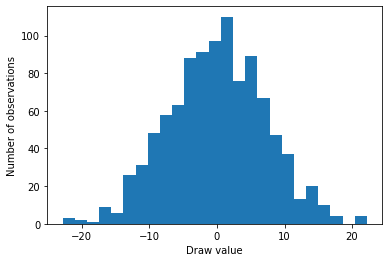
\includegraphics[scale=0.6]{Plots/hist_Q1.png}
% \centering
% \caption{Histogram of addition of 1000 draws from two Gaussian distributions}
% \label{fig:hist_Q1}
% \centering
% \end{figure}

\subsubsection{Code for problem 1}
\begin{lstlisting}
import pandas as pd
import matplotlib.pyplot as plt
import numpy as np
import scipy
from zipfile import ZipFile 
import seaborn as sb
import os
from sklearn.linear_model import LinearRegression

file_name = "Lab2_data.zip"

with ZipFile(file_name, 'r') as zip: 
    zip.extractall() 

header_list = ["X0", "X1", "X2", "X3", "X4"]
df1 = pd.read_csv("DF1", header = None, names = header_list)
df1 = df1.iloc[1:]
df1 = df1.drop(columns = ["X0"])
print(df1.head())

#df1.drop(0, axis=1)

from pandas.plotting import scatter_matrix
scatter_matrix(df1, alpha=0.2, figsize=(12, 12))

sb.pairplot(df1)

print("From the scatterplots, it appears that column 0 and column 2 
are correlated, as well as column 1 and column 3. Note that the original
column zero has been dropped as it is just the observation number.\n")

print("The formula for the covariance matrix of a dataset is given by:
E[XX^T] - E[X](E[X]^T)")

print("The covariance matrix of the dataset is: ")
print(np.cov(np.transpose(df1)))


print("Let Z = (X1, X2, X3), where K is the correlation matrix.")
print("For the required relations, we have the correlation matrix as
K = ([1, 0, 0], [0, 1, -1], [0, -1, 1])")

K = [[1, 0, 0], [0, 1, -1], [0, -1, 1]]
cov_obs = []
for i in range(998):
    Obs= np.random.multivariate_normal(mean = [0,0,0], cov=K, size = i+2)
    cov_mat = np.cov(np.transpose(Obs))
    cov_obs.append(cov_mat[2,1])
print(cov_obs)


fig, ax = plt.subplots()
ax.set_xlabel('Number of samples') 
ax.set_ylabel('Covariance')
# set the xlim
ax.set_xlim(3, 1000)
dim = np.arange(3,1001,1);
actual_cov = [-1]*998
ax.plot(dim, cov_obs, label="covariance") 
ax.plot(dim, actual_cov, "r", label="true covariance") 
legend = ax.legend(loc='best', shadow=False, fontsize='small')
plt.show()
\end{lstlisting}

%-------------------------------------------------------

\subsection{Problem 2}

\textbf{Outliers}\\

Consider the two-dimensional data in DF2 in Lab2 Data.zip. Look at a scatter plot of the data. It contains two points that look like potential outliers. Which one is "more" outlying? Propose a transformation of the data that makes it clear that the point at $(-1, 1)$ is more outlying than the point at (5.5, 5), even though the latter point is "farther away" from the nearest points. Plot the data again after performing this transformation. Provide discussion as appropriate to justify your choice of transformation.\\

\noindent\textit{Hint: if y comes from a standard Gaussian in two dimensions (i.e., with covariance equal to the two by two identity matrix), and
\begin{equation*}
    Q = \begin{pmatrix}2 & \frac{1}{2}\\\frac{1}{2} & 2\end{pmatrix},
\end{equation*}
what is the covariance matrix of the random variable z = Qy? If you are given z, how would you create a random Gaussian vector with covariance equal to the identity, using z?}\\

\subsubsection{Solution to problem 2}



\subsubsection{Code for problem 2}
\begin{lstlisting}

\end{lstlisting}

%-------------------------------------------------------

\subsection{Problem 3}

\textbf{Even more standard error}\\

In one of the written exercises below, you derive an expression for what is called the Standard Error: where $\beta$ denotes the "truth,", $\hat{\beta}$ denotes the value we compute using least squares linear regression, and $Z$ and $e$ are as in the exercise below, you find:
\begin{equation*}
    \hat{\beta} - \beta = Ze
\end{equation*}

If we know the distribution of the noise (the distribution generating the noise vectors, $e_i$), then we know the distribution for the error, ($\hat{\beta} - \beta$). This allows us to answer the question: if we solve a regression and obtain value $\hat{\beta}$, how can we tell if it is statistically significant? The answer is: we compare the size of $\hat{\beta}$ to the spread introduced by the noise (i.e., the standard error), and we ask: what is the likelihood that the true $\beta = 0$, and what we observed was purely due to the noise.\\

If the noise is Gaussian (normal), i.e., $e_i \sim N(0, \sigma^2)$, and if the values of the $x_i$ are normalized, then we expect error of the size $\sigma/\sqrt(n)$, as this is roughly the standard deviation of the expression for the error that you derive above. This means: if you have twice the data points, you should expect the error to be reduced by about 1.4 (the formula says that the standard deviation of the error would decrease by a factor of $1/\sqrt(2)$).

Compute this empirically, as follows: We will generate data for a regression problem, solve it, and see what the error is: Generate data as follows: $xi \sim N(0, 1), e_i \sim N(0, 1)$. Generate $y$ by $y_i = \beta_0 + x_i\beta + e_i$, where $\beta_0 = -3$ and $\beta = 0$. Note that since $\beta = 0$, this means that y and x are unrelated! The question we are exploring here is as follows: when we solve a regression problem, we are not going to find $\hat{\beta} = 0$ - we will find that $\hat{beta}$ takes some other values, hopefully close to zero. How do we know if the value of $\hat{\beta}$ we get is statistically meaningful?
\begin{itemize}
    \item By creating fresh data and each time computing $\hat{\beta}$ and recording $\hat{\beta} - \beta$, compute the empirical standard deviation of the error for n = 150. By running a linear regression of y vs. noise, we find $\hat{\beta} = -0.15$. Given your empirical computation of the standard deviation of the error, how significant is the value -0.15
    \item Now repeat the above experiment for different values of n. Plot these values, and on the same plot, plot $1/sqrt(n)$. How is the fit?
\end{itemize}

\subsubsection{Solution to problem 3}



\subsubsection{Code for problem 3}
\begin{lstlisting}

\end{lstlisting}


%-------------------------------------------------------

\subsection{Problem 4}

\textbf{Names and frequencies}\\

The goal of this exercise is for you to get more experience with Pandas, and to get a chance to explore a cool data set. Download the file Names.zip from Canvas. This contains the frequency of all names that appeared more than 5 times on a social security application from 1880 through 2015.

\begin{itemize}
    \item Write a program that on input $k$ and $XXXX$, returns the top k names from year $XXXX$.
    \item Write a program that on input \textbf{Name} returns the frequency for men and women of the name \textbf{Name}.
    \item It could be that names are more diverse now than they were in 1880, so that a name may be relatively the most popular, though its frequency may have been decreasing over the years. Modify the above to return the relative frequency. Note that in the next coming lectures we will learn how to quantify diversity using entropy.
    \item Find all the names that used to be more popular for one gender, but then became more popular for another gender.
\end{itemize}

\subsubsection{Solution to problem 4}



\subsubsection{Code for problem 4}
\begin{lstlisting}

\end{lstlisting}

%-------------------------------------------------------




\end{document}
